\textbf{See the instruction for questions \inteval{\value{question}+1} to \inteval{\value{question}+3}.}

\begin{figure}[H]
    \center
    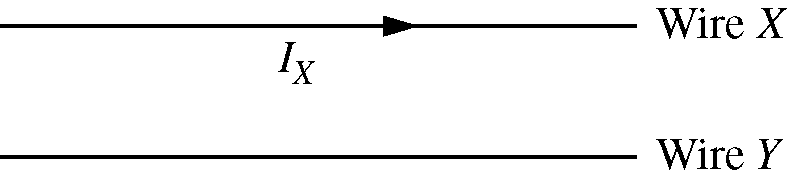
\includegraphics[scale=0.25]{images/img-003-005.png}
\end{figure}

Two long, straight, parallel wires are held fixed, as shown above. A voltage is applied to wire $X$, creating a current $I_{X}$ to the right, and the wire experiences a magnetic force of magnitude $F_{B}$ toward wire $Y$.

% Multiple Choice Question 6
\begin{questions}\setcounter{question}{5}\question
Assuming the resistance of wire $X$ is constant, which of the following graphs correctly illustrates the magnitude of the magnetic force $F$ on wire $X$ as a function of the voltage $V$ applied to the wire?

\begin{oneparchoices}
\choice \adjustbox{valign=t}{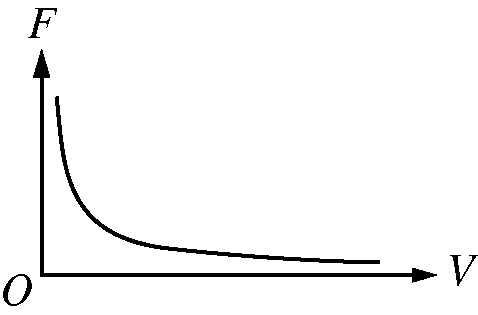
\includegraphics[scale=0.25]{images/img-003-006.png}}
\choice \adjustbox{valign=t}{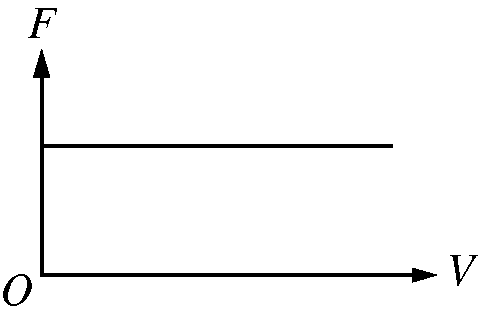
\includegraphics[scale=0.25]{images/img-003-007.png}}
\choice \adjustbox{valign=t}{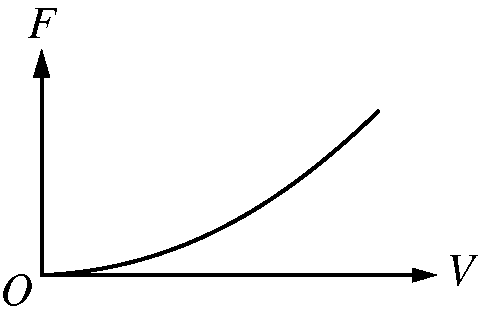
\includegraphics[scale=0.25]{images/img-003-008.png}}
\choice \adjustbox{valign=t}{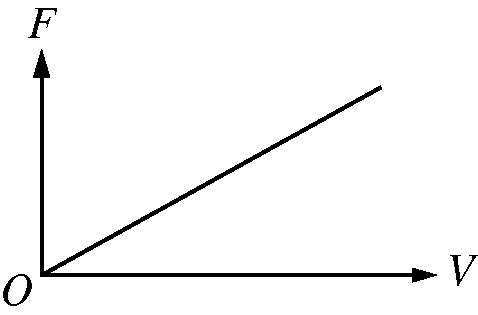
\includegraphics[scale=0.25]{images/img-003-009.png}}
\choice \adjustbox{valign=t}{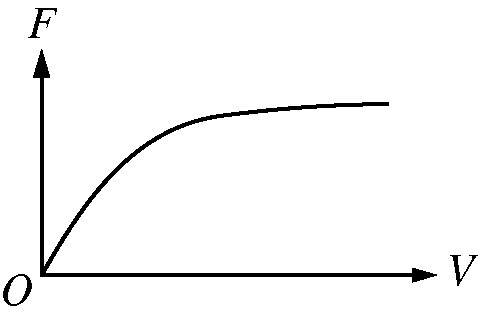
\includegraphics[scale=0.25]{images/img-003-010.png}}
\end{oneparchoices}\end{questions}

% Multiple Choice Question 7
\begin{questions}\setcounter{question}{6}\question
Which of the following could be true of wire $Y$?
\begin{enumerate}
    \item It carries a current in the same direction as the current in wire $X$.
    \item It experiences a force directed away from wire $X$.
    \item It experiences a force of different magnitude than the force on wire $X$.
\end{enumerate}

\begin{oneparchoices}
\choice None
\choice I only
\choice II only
\choice III only
\choice I or II
\end{oneparchoices}\end{questions}

% Multiple Choice Question 8
\begin{questions}\setcounter{question}{7}\question
If the distance between the two wires is tripled, what is the magnitude of the new magnetic force exerted on wire $X$ ?

\begin{oneparchoices}
\choice $F_{B} / 9$
\choice $F_{B} / 3$
\choice $F_{B}$
\choice $3 F_{B}$
\choice $9 F_{B}$
\end{oneparchoices}\end{questions}

